\chapter{Pruebas} \label{pruebas}

En este punto deberíamos tener un sistema totalmente funcional, pero nos falta comprobar la calidad del mismo. La calidad de nuestro sistema vendrá determinada por la calidad de cada uno de sus elementos. En este apartado se realizarán pruebas sobre las principales partes funcionales del sistema. Estas pruebas irán variando según la funcionalidad de la parte examinada.

\section{Pruebas sobre la interfaz web}

La interfaz web es el conjunto de elementos que se muestran al usuario a través del navegador. Las pruebas aplicadas sobre esta parte del sistema son simples, consisten en un recorrido por todos los posibles caminos existentes en la interfaz web. Durante este recorrido por la interfaz web se verá si hay zonas poco intuitivas, si hay fallos en los redireccionamientos, si hay caminos que no desembocan en alguna de las interfaces del chatbot, entre otros fallos a revisar en la interfaz.

Para obtener unos resultados más objetivos, las pruebas han sido ejecutadas por personas externas al desarrollo del proyecto. A cada uno de los usuarios que ha realizado la prueba, la cual consistía en un uso libre del sistema durante 10 minutos, al finalizar el término establecido se le realizaba una pregunta sobre la puntuación que le daba al sistema del 0 al 10.

La puntuación media obtenida para nuestro sistema ha sido de un 7 sobre 10. Los comentarios de los usuarios destacan que la interfaz web es bastante funcional, pero que la parte que le hacía perder nota era su estética, que podría ser mejorable añadiendo diseños más actuales.

Para tener más datos objetivos con los que evaluar la calidad de la interfaz web, se ha efectuado un test de accesibilidad a la interfaz en su totalidad. Hoy en día hay cierta tendencia a mejorar la accesibilidad para mejorar el empleo de las interfaces web por parte de las personas con alguna discapacidad que les dificulte el uso de las mismas. Para obtener una interfaz con una gran nivel de accesibilidad existen las pautas de accesibilidad al contenido web (Web Content Accessibility Guidelines - WCAG). Estas pautas son unos documentos que explican cómo hacer el contenido web de nuestro sistema accesible para personas con discapacidad. Actualmente, existen muchos comprobadores online para obtener el nivel de accesibilidad de nuestro sistema. Existen distintos niveles de conformidad para categorizar nuestro sistema, estos niveles son el nivel A, AA y AAA. Los niveles mencionados van desde menos restrictivos a más restrictivos. El nivel AA contiene las restricciones del nivel A y las propias del nivel AA. Y de igual forma pasa con el nivel AAA, que contiene las restricciones de los dos niveles anteriores y las propias del nivel AAA.

El comprobador online que he utilizado para analizar la accesibilidad de nuestra interfaz web ha sido \href{https://www.siteimprove.com/toolkit/accessibility-checker/?utm_campaign=southeurope_en_ppc_accessibility&utm_medium=ppc&utm_source=google&utm_content=web-accessibility&utm_term=website}{Siteimprove}. La puntuación que se ha obtenido de la interfaz web con este comprobador online se puede comprobar en la Tabla \ref{tab:punt_accesibilidad_interfaz_web}. En esta tabla se puede ver tanto la puntuación media de la interfaz web como la puntuación desglosada de cada sección de la interfaz web. La puntuación de cada página se divide en cuatro puntuaciones distintas. Estas cuatro puntuaciones son la puntuación general de cada página y las tres puntuaciones de los niveles A, AA y AAA.


\begin{table}[h]
\centering
\resizebox{\textwidth}{!}{%
\begin{tabular}{l|c|c|c|c|}
\cline{2-5}
 &
  \cellcolor[HTML]{C0C0C0}\textbf{\begin{tabular}[c]{@{}c@{}}Puntuación general \\ de la página\end{tabular}} &
  \cellcolor[HTML]{C0C0C0}\textbf{\begin{tabular}[c]{@{}c@{}}Puntuación \\ nivel A\end{tabular}} &
  \cellcolor[HTML]{C0C0C0}\textbf{\begin{tabular}[c]{@{}c@{}}Puntuación \\ nivel AA\end{tabular}} &
  \cellcolor[HTML]{C0C0C0}\textbf{\begin{tabular}[c]{@{}c@{}}Puntuación \\ nivel AAA\end{tabular}} \\ \hline
\multicolumn{1}{|l|}{\cellcolor[HTML]{C0C0C0}\textbf{Página principal}}              & 69.9 / 100  & 84.5 / 100 & 71.3 / 100  & 53.9 / 100 \\ \hline
\multicolumn{1}{|l|}{\cellcolor[HTML]{C0C0C0}\textbf{Actividad del chatbot}}         & 77.1 / 100  & 84.5 / 100 & 71.3 / 100  & 75.6 / 100 \\ \hline
\multicolumn{1}{|l|}{\cellcolor[HTML]{C0C0C0}\textbf{Página de captura de imágenes}} & 69.1 / 100  & 84.7 / 100 & 71.3 / 100  & 51.2 / 100 \\ \hline
\multicolumn{1}{|l|}{\cellcolor[HTML]{C0C0C0}\textbf{Interfaz del chatbot}}          & 61.2 / 100  & 91.1 / 100 & 57.4 / 100  & 34.9 / 100 \\ \hline
\rowcolor[HTML]{FFFFC7} 
\multicolumn{1}{|l|}{\cellcolor[HTML]{C0C0C0}\textbf{Interfaz web}}                  & 69.33 / 100 & 86.2 / 100 & 67.83 / 100 & 53.9 / 100 \\ \hline
\end{tabular}%
}
\caption{Puntuación de accesibilidad de la interfaz web}
\label{tab:punt_accesibilidad_interfaz_web}
\end{table}

Basándonos en las puntuaciones mostradas en la Tabla \ref{tab:punt_accesibilidad_interfaz_web}, podemos indicar que el nivel de accesibilidad no es muy alto en general en nuestra interfaz web. Sobre todo destaca la baja puntuación en los niveles más restrictivos. Se consideraría que el nivel de accesibilidad es aceptable si se llega a tener una puntuación media de 85 sobre 100, en al menos los dos primeros niveles. Por lo tanto, la accesibilidad de nuestro sistema podría ser un punto a mejorar, sobre todo si el volumen de usuarios que van a usar nuestro sistema está formado por un gran número de usuarios con discapacidad. De todas maneras, el aumento de la accesibilidad nunca será inconveniente para la experiencia de los usuarios con la interfaz, sino todo lo contrario. Aunque, por supuesto, sí que conllevaría un aumento de la carga de trabajo a la hora de implementar la interfaz web.

\section{Pruebas sobre la deducción de edad}

Otra parte fundamental del sistema es la deducción de la edad. Como se indicó en el apartado de implementación del Modelo, se ha hecho uso de un modelo pre entrenado para realizar esta deducción. Para comprobar la calidad de este modelo, y en consecuencia la calidad del sistema para deducir la edad, se han efectuado una serie de deducciones con imágenes extraídas de una base de imágenes libres llamada \href{https://www.pexels.com/es-es/}{Pexels}. Las imágenes que se han extraído de esta base de imágenes se pueden ver en la Figura \ref{fig:img_prueba_caras}. Como se puede apreciar, se han extraído imágenes de caras de personas de distintas edades para intentar forzar al modelo y ver su verdadera calidad.

\begin{figure}
    \centering
    \subfloat[]{
    \begin{subfigure}
        \centering
        
\includegraphics[width=0.4\textwidth]{imagenes/08_Pruebas/pexels-simon-robben-614810.jpg}
        \label{subfig:caraA}
    \end{subfigure}
    }
    \subfloat[]{
    \begin{subfigure}
        \centering
        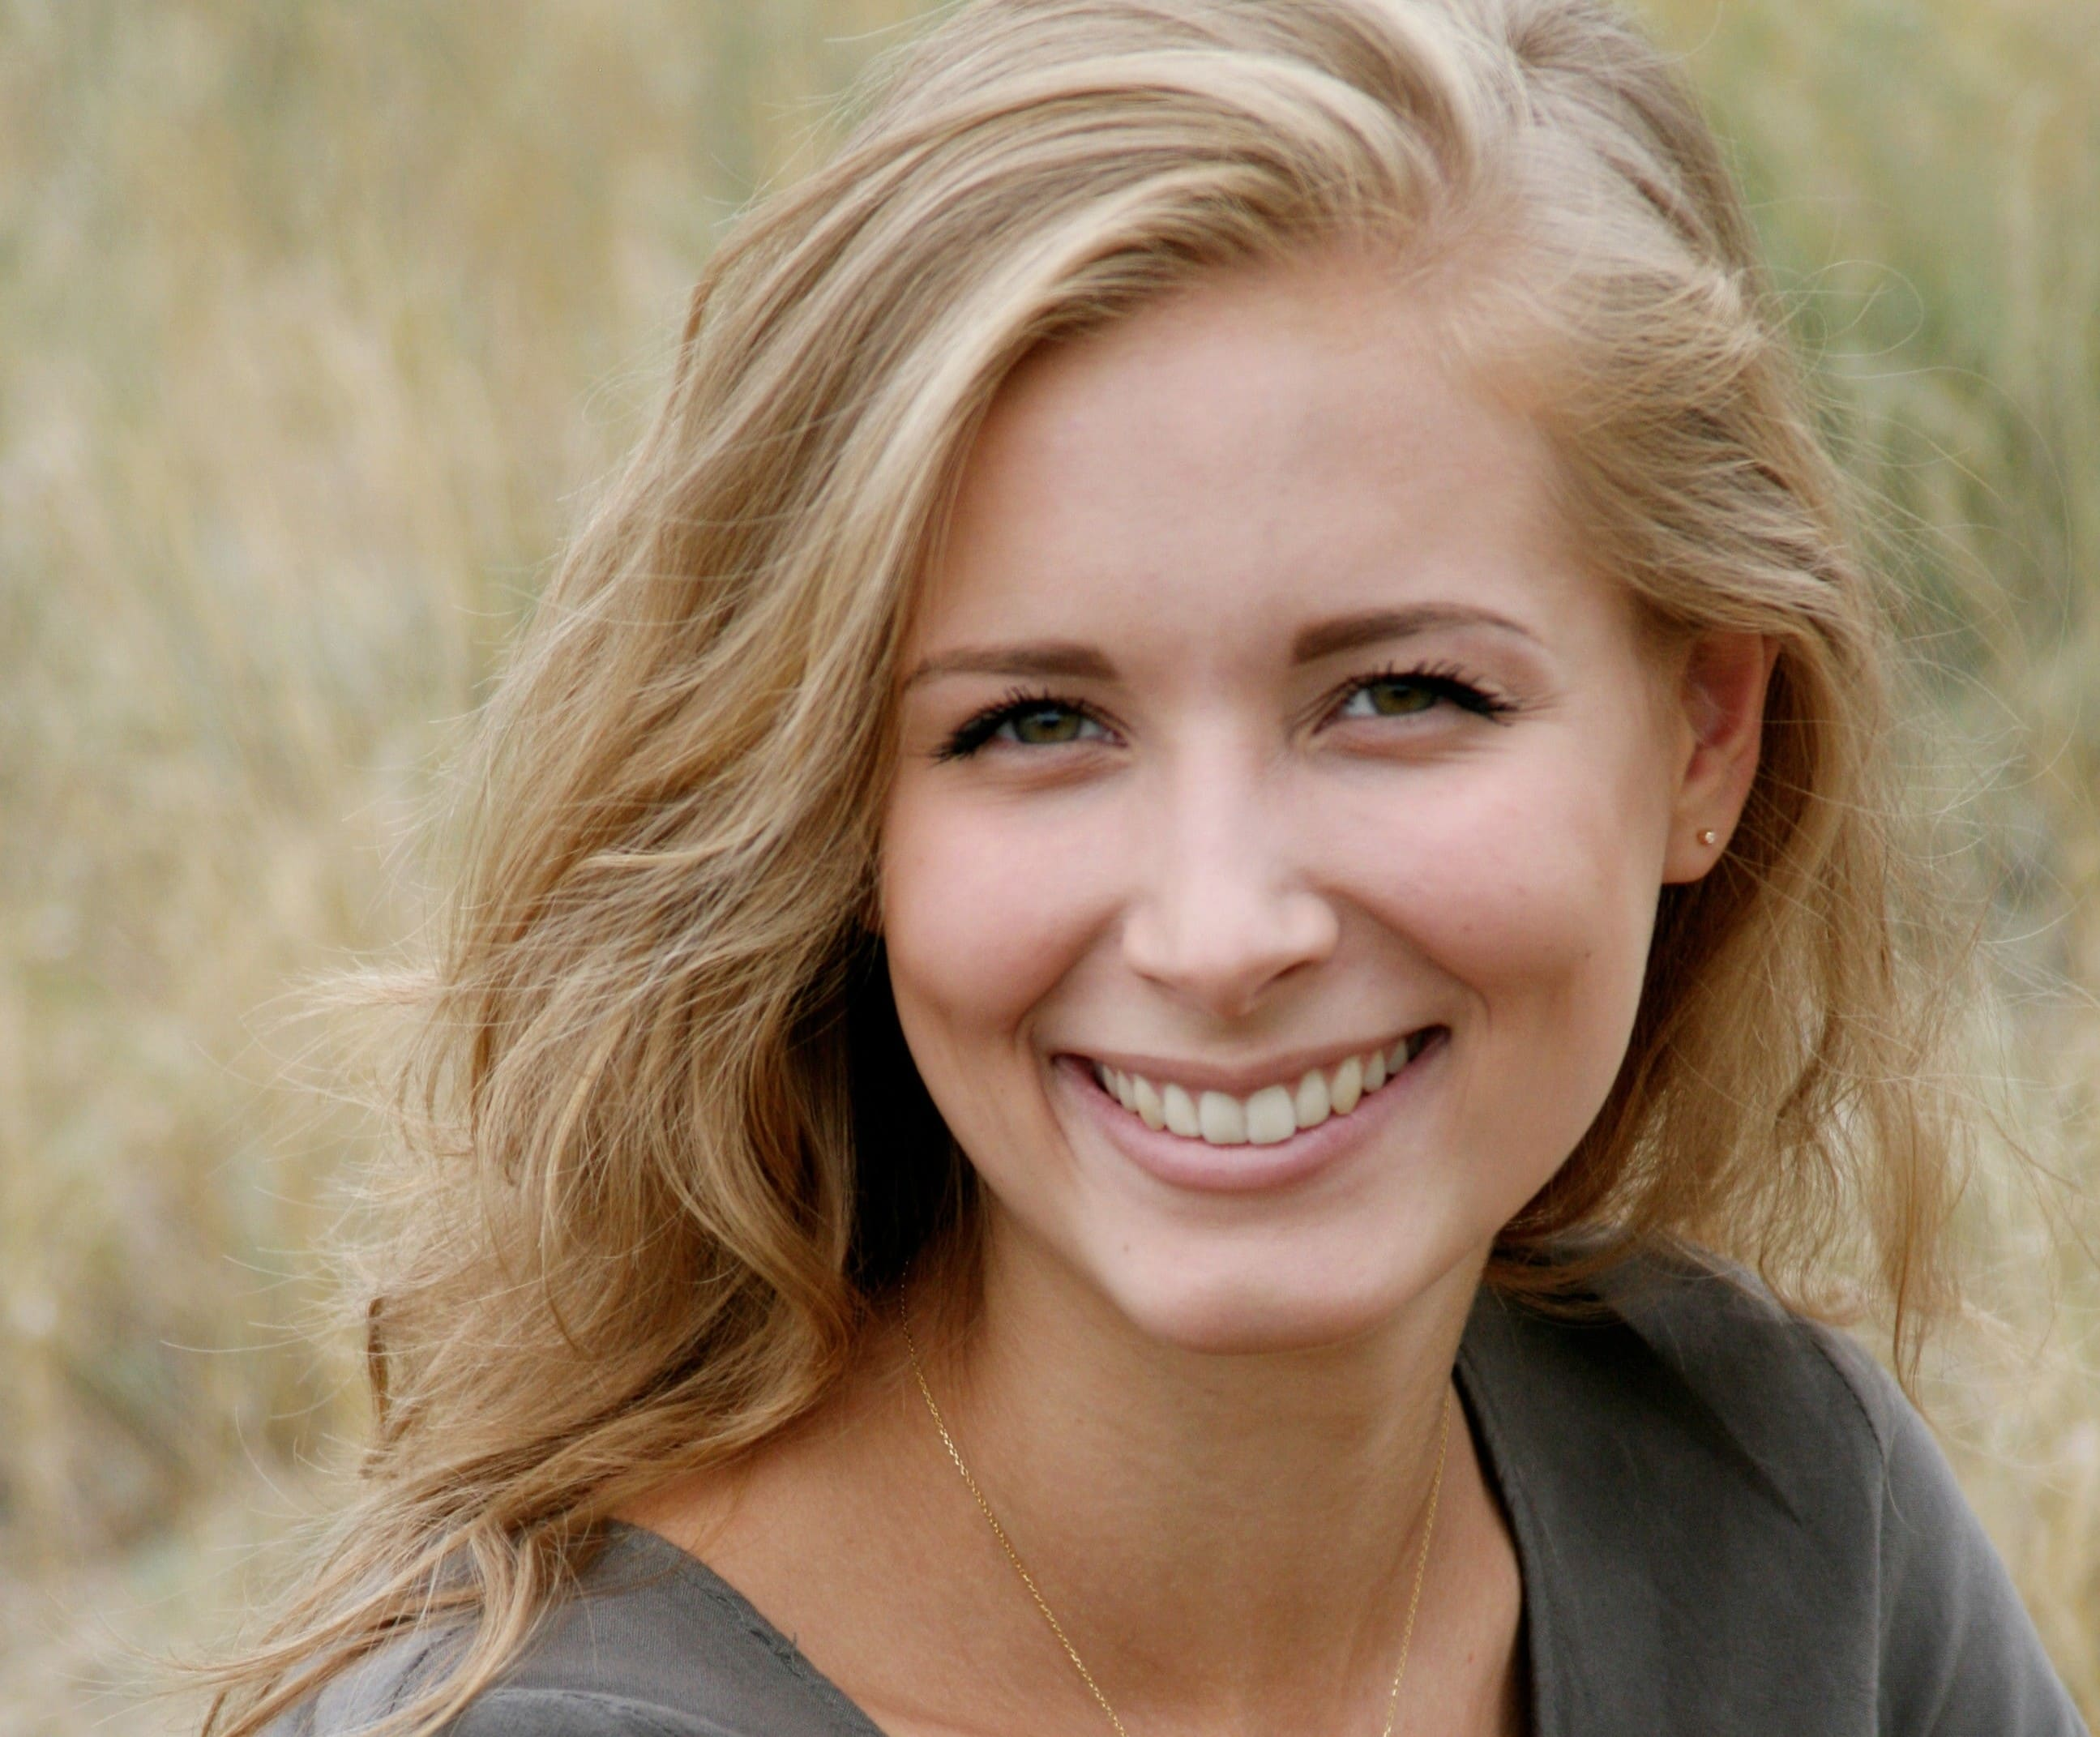
\includegraphics[width=0.4\textwidth]{imagenes/08_Pruebas/pexels-pixabay-38554.jpg}
        \label{subfig:caraB}
    \end{subfigure}
    }
    \hfill
    \subfloat[]{
    \begin{subfigure}
        \centering
        
\includegraphics[width=0.4\textwidth]{imagenes/08_Pruebas/pexels-bess-hamiti-35537.jpg}
        \label{subfig:caraC}
    \end{subfigure}
    }
    \subfloat[]{
    \begin{subfigure}
        \centering
        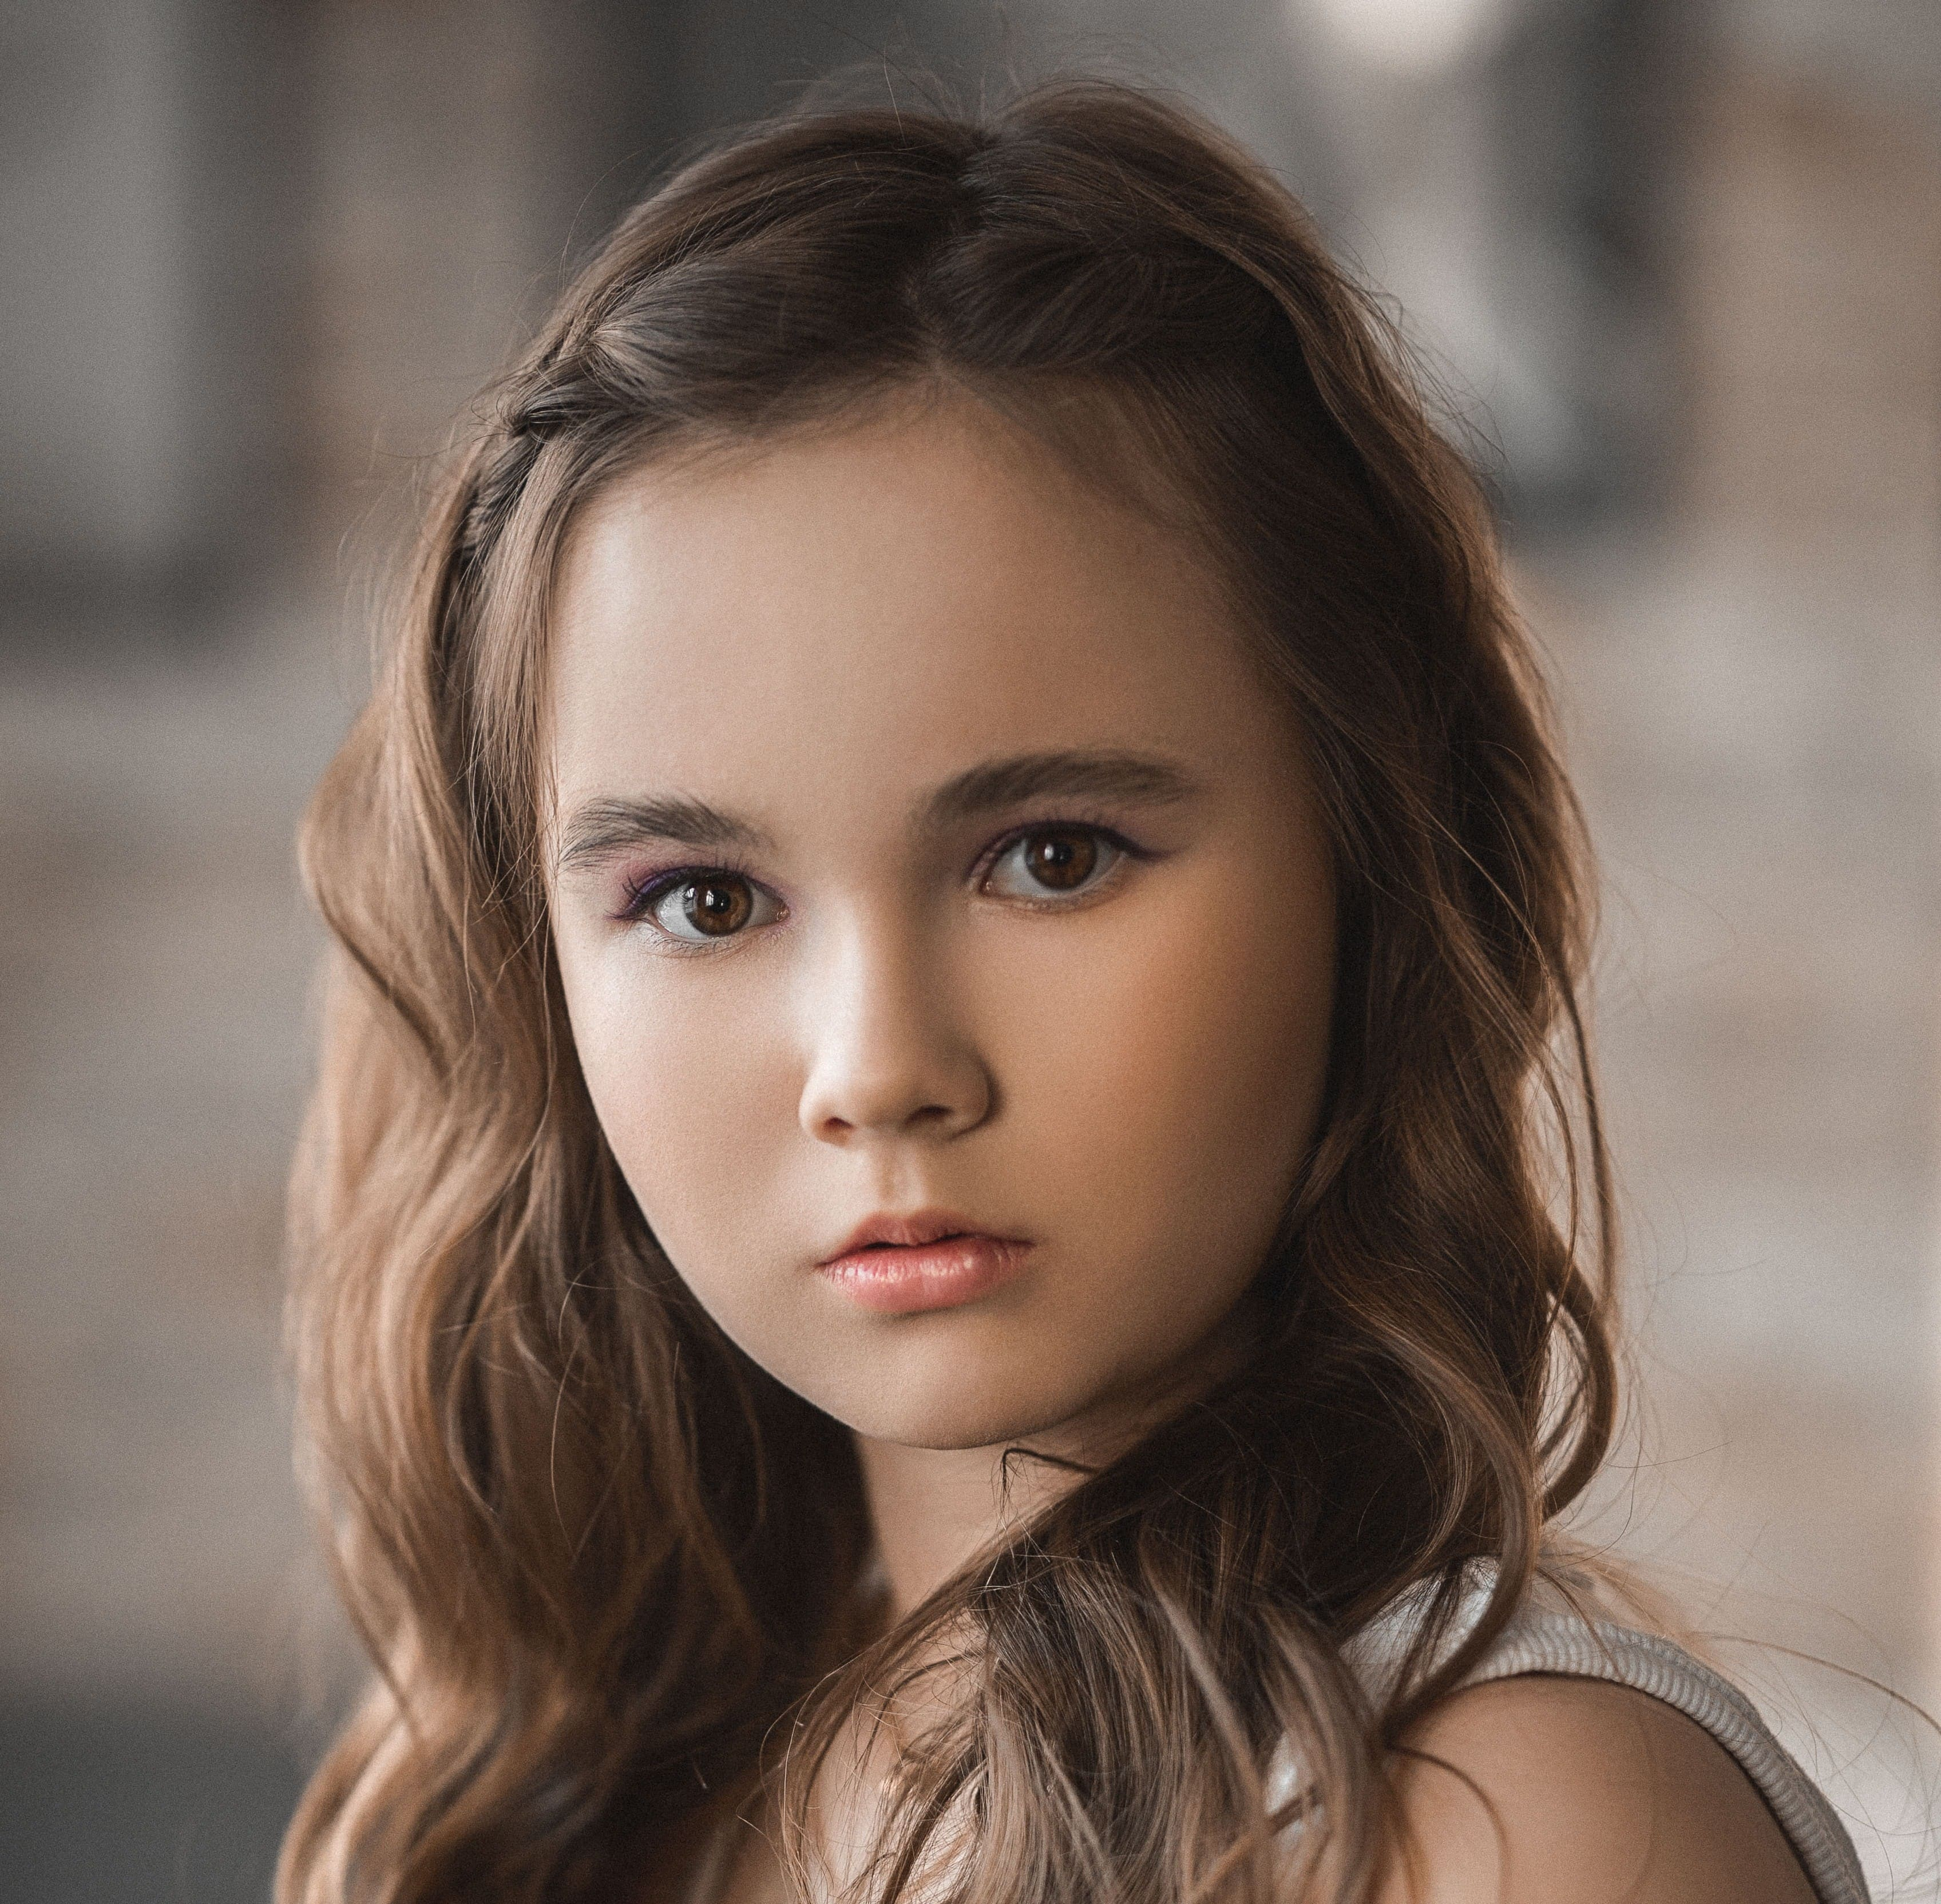
\includegraphics[width=0.4\textwidth]{imagenes/08_Pruebas/pexels-владимир-васильев-9402457.jpg}
        \label{subfig:caraD}
    \end{subfigure}
    }
    \hfill
    \subfloat[]{
    \begin{subfigure}
        \centering
        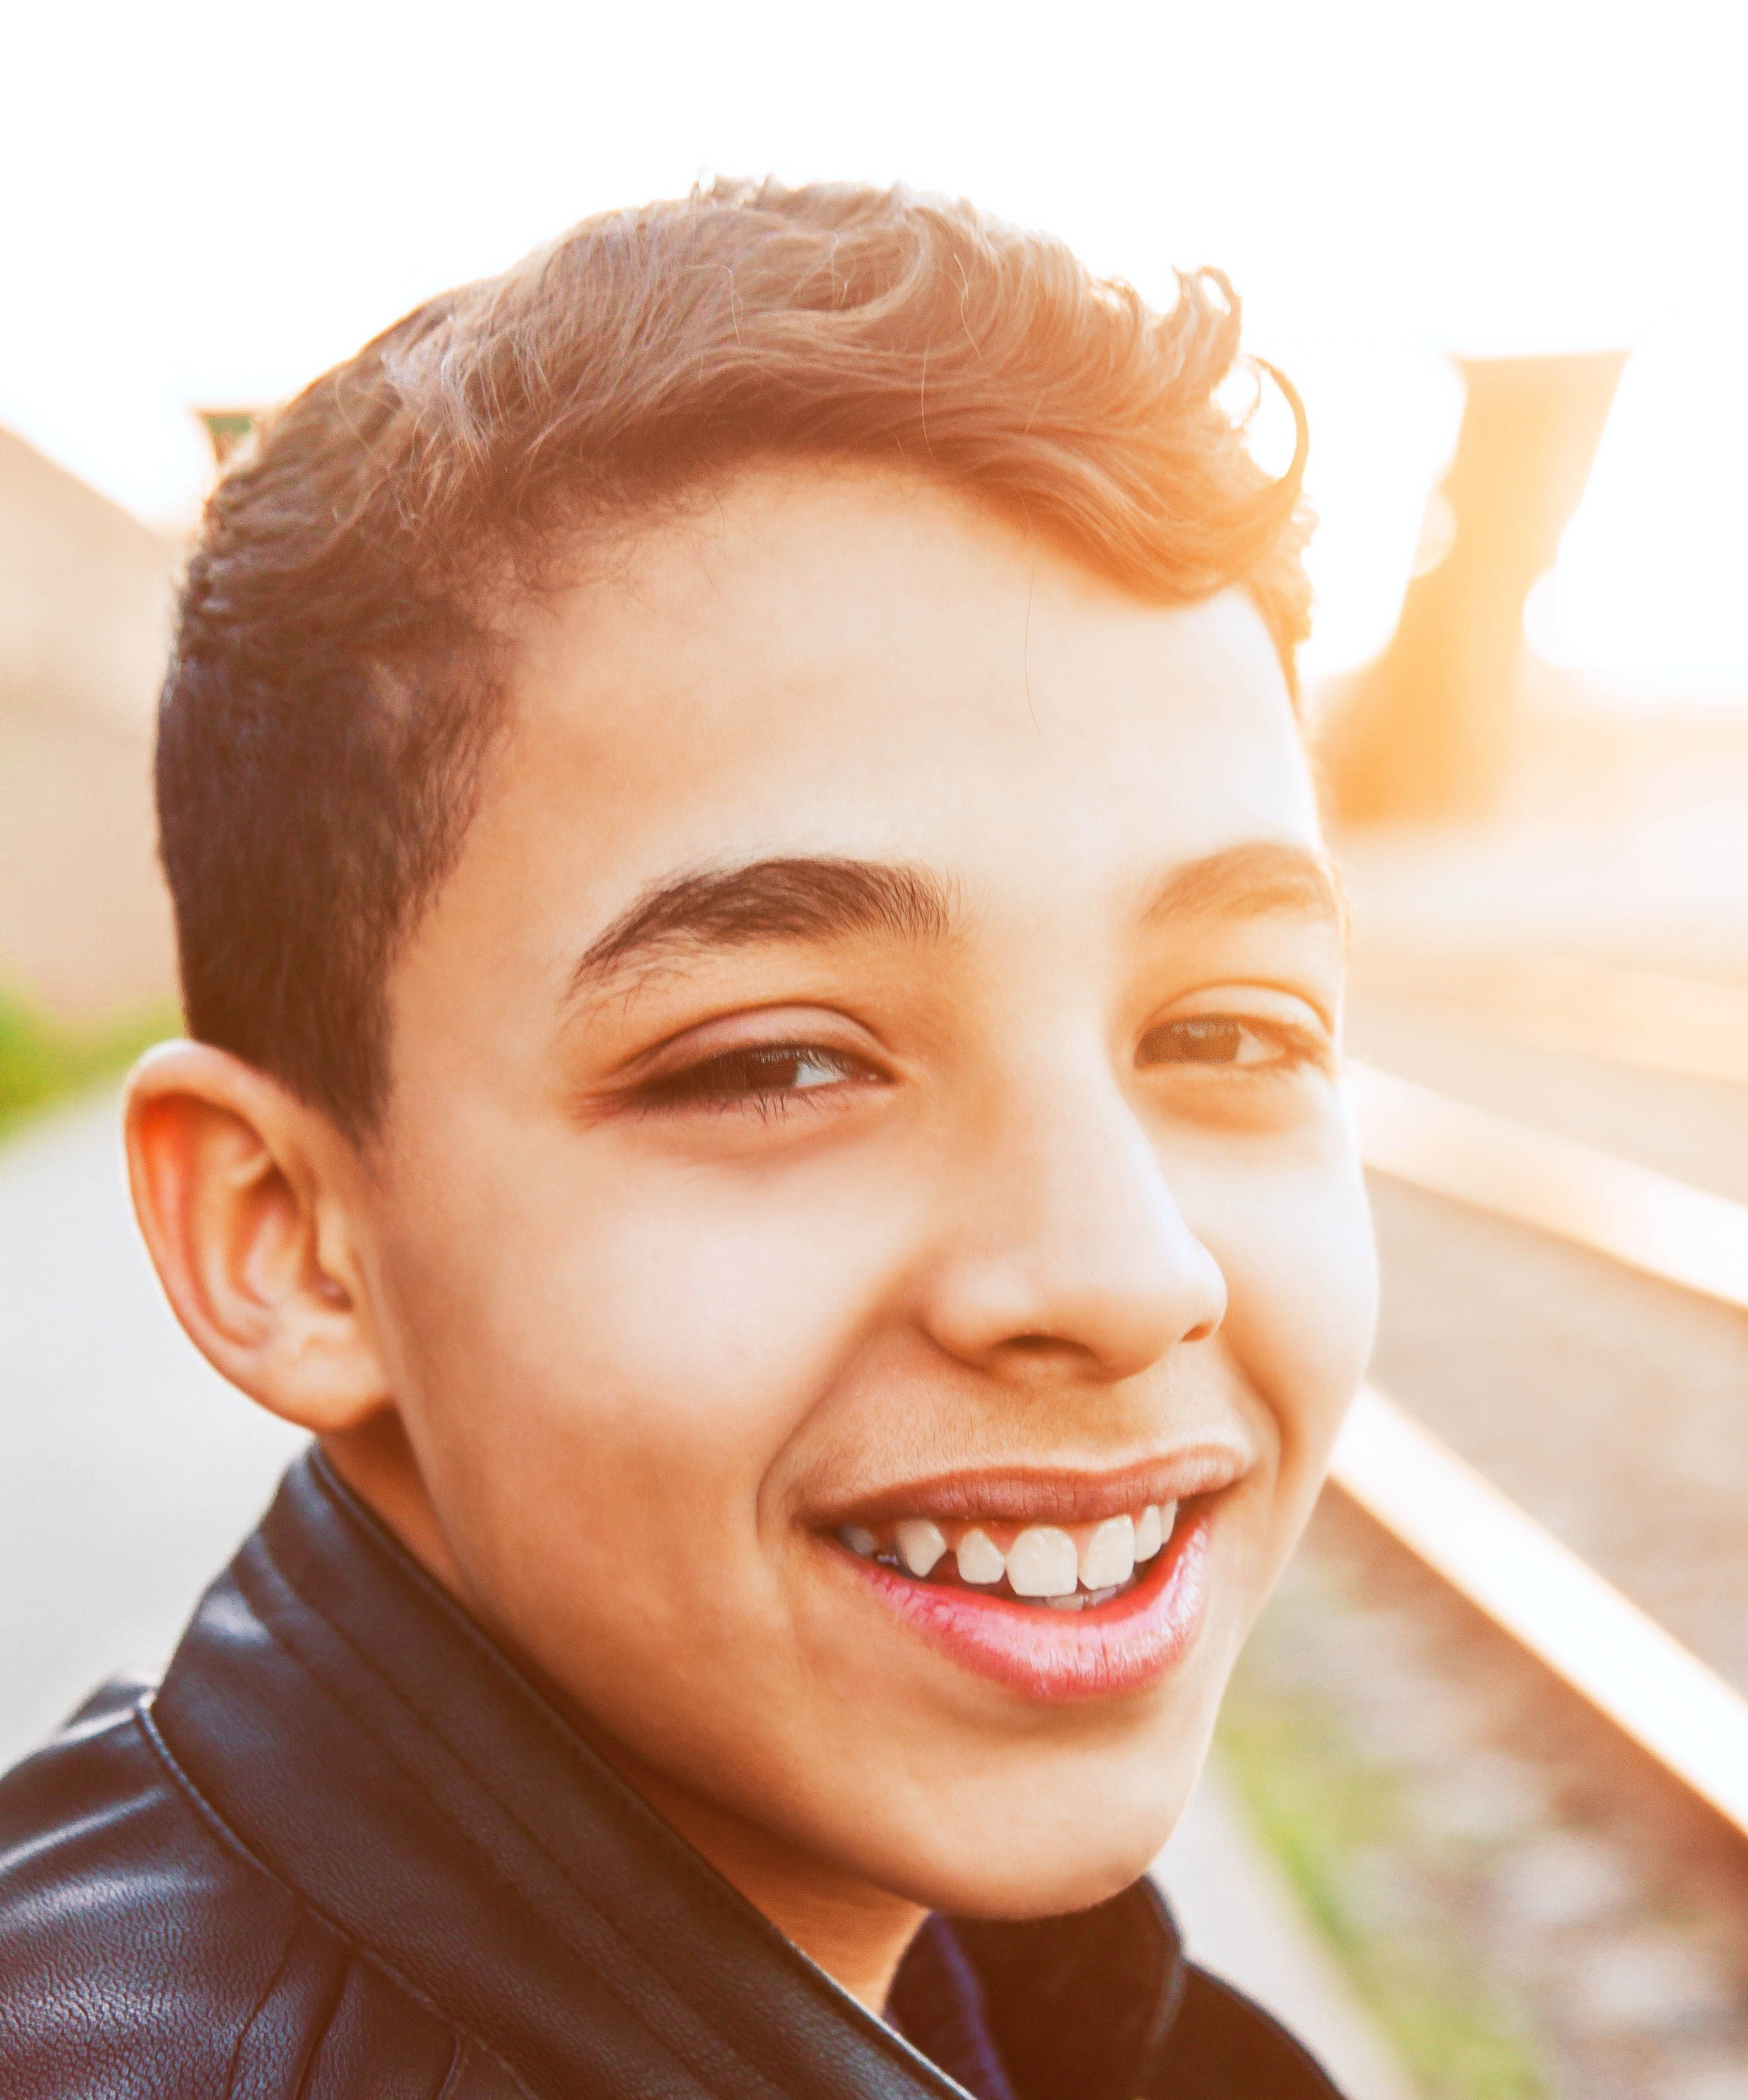
\includegraphics[width=0.4\textwidth]{imagenes/08_Pruebas/pexels-mohamedamine-abbas-2588337.jpg}
        \label{subfig:caraE}
    \end{subfigure}
    }
    \subfloat[]{
    \begin{subfigure}
        \centering
        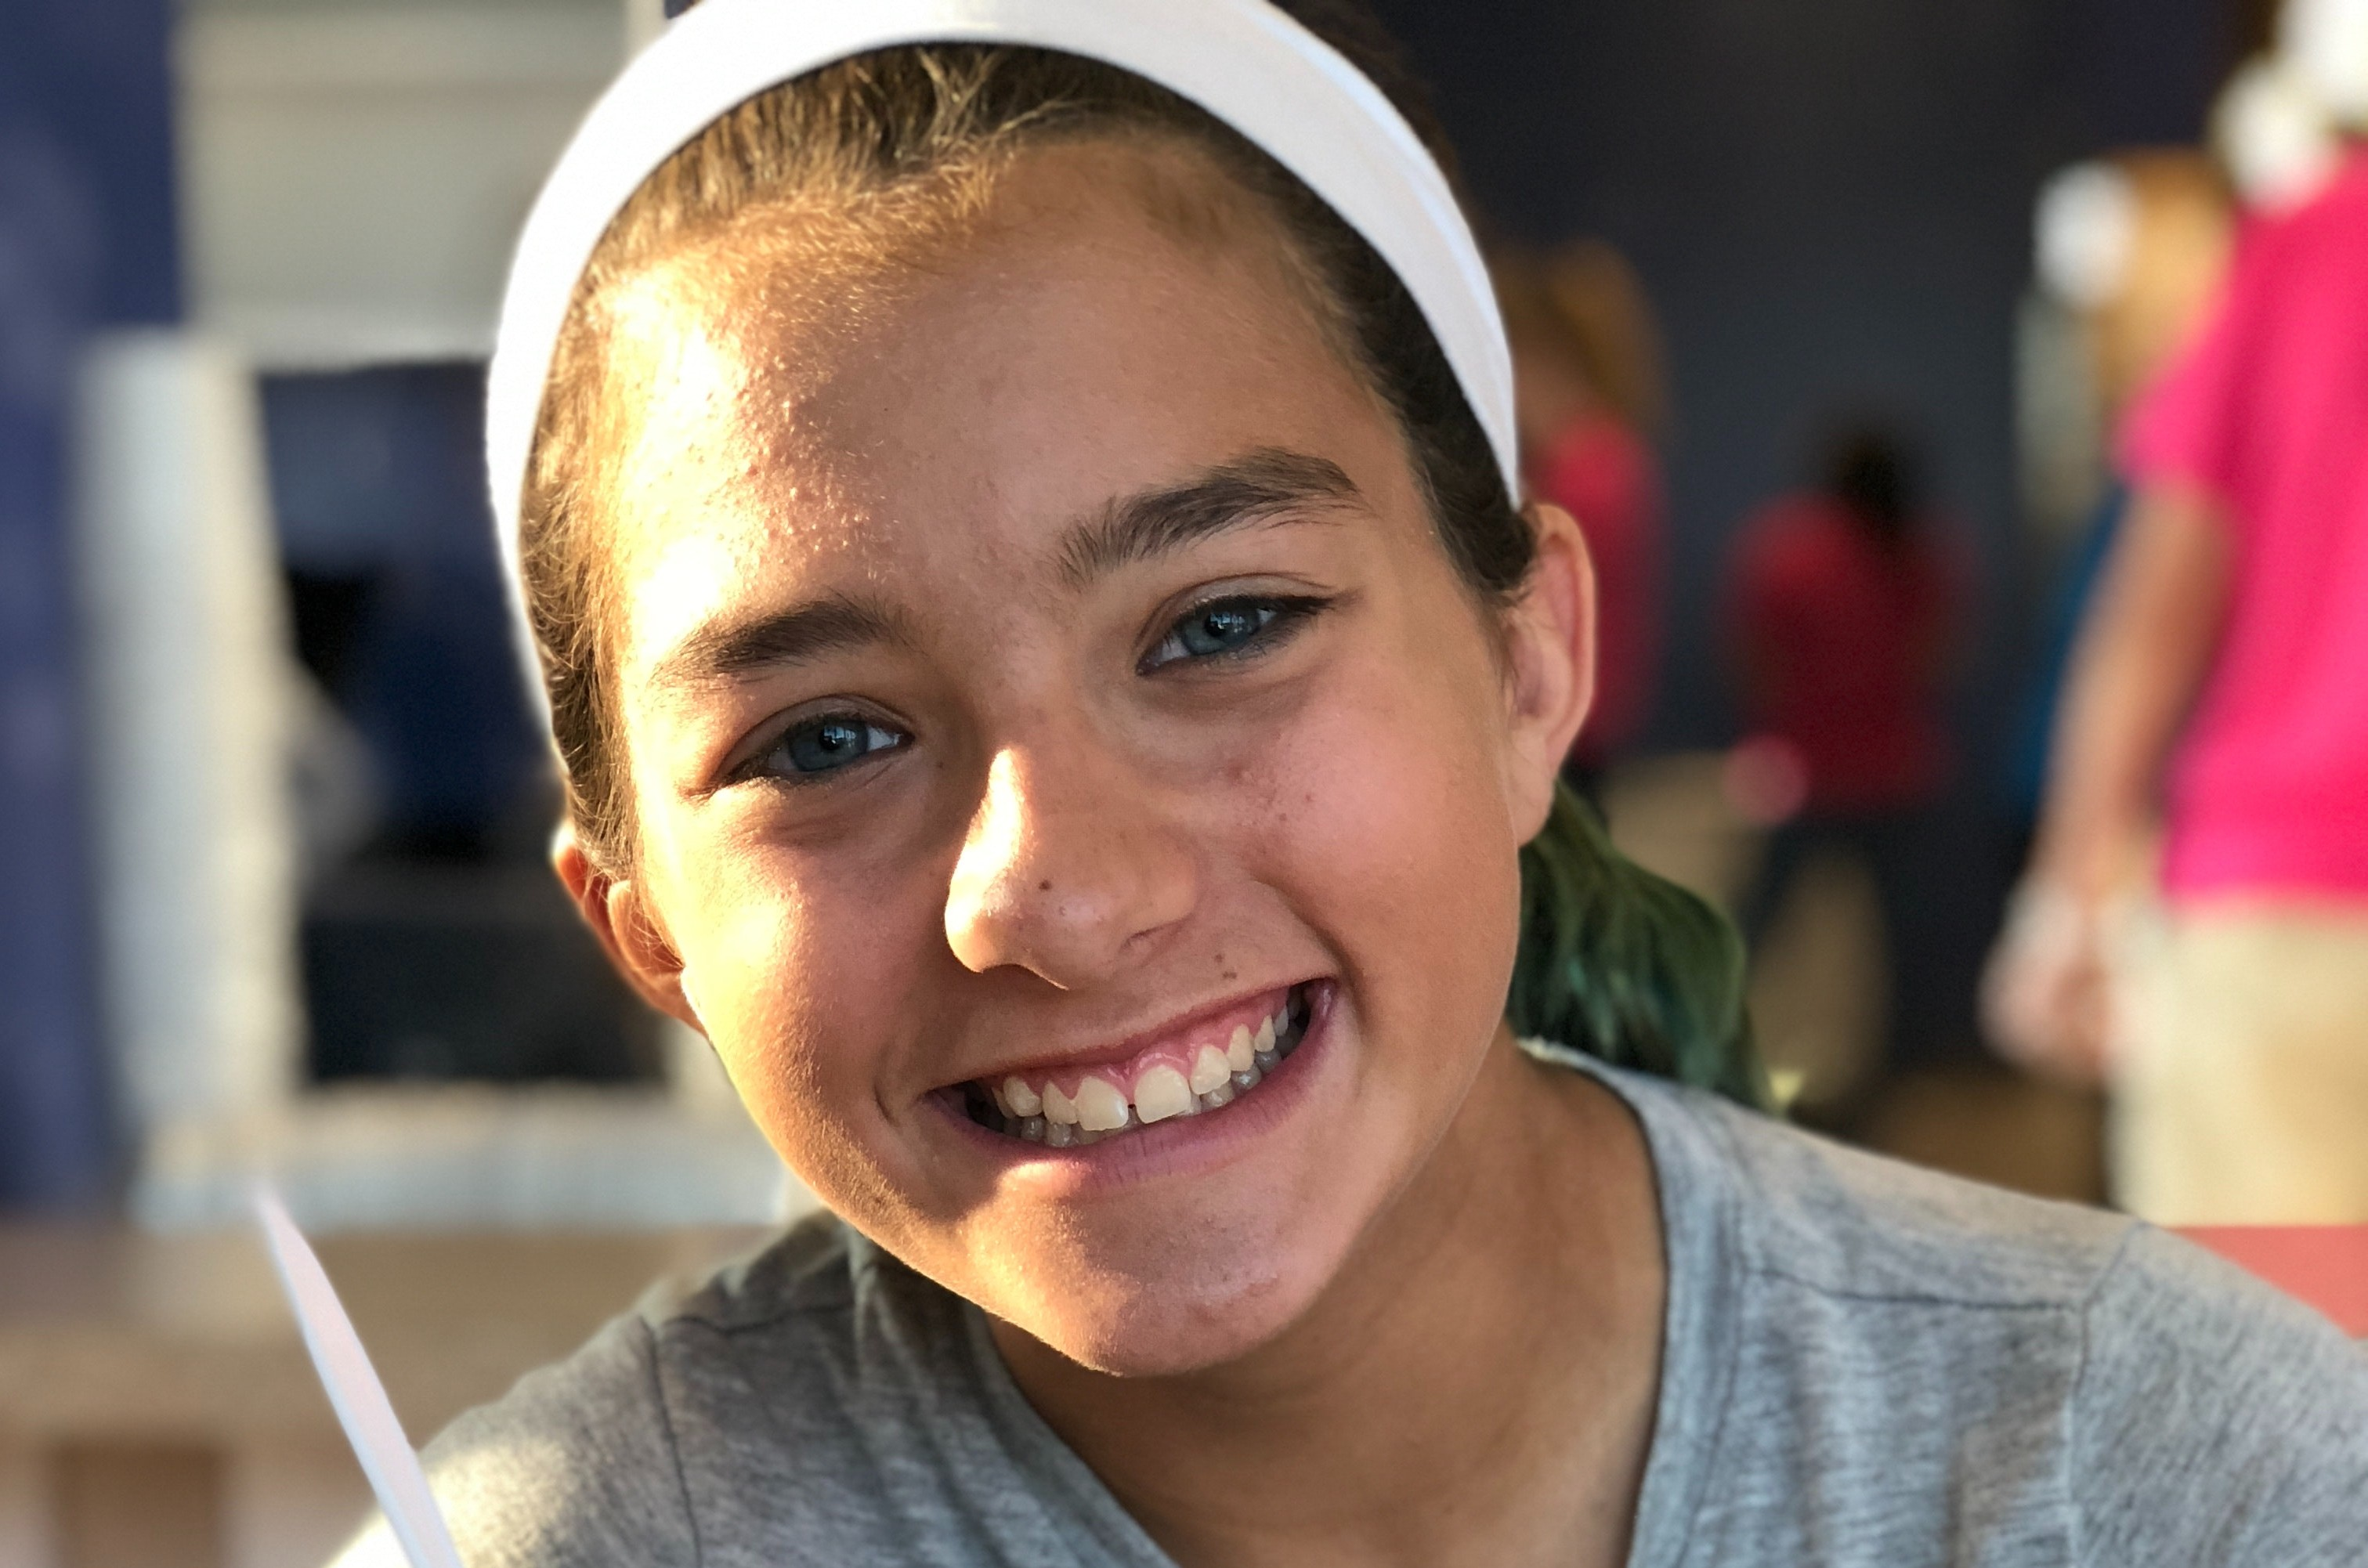
\includegraphics[width=0.4\textwidth]{imagenes/08_Pruebas/pexels-david-mcbee-1332945.jpg}
        \label{subfig:caraF}
    \end{subfigure}
    }
\caption{Imágenes de las caras usadas para las pruebas}
\label{fig:img_prueba_caras}
\end{figure}


Tal y como se expuso en el apartado de implementación de esta sección de deducción, el modelo pre entrenado que estamos utilizando clasifica las edades dentro de unos ciertos rangos. El rango más comprometido es el rango que va desde los 10 hasta los 19 años, ya que para nuestro sistema una persona deja de ser niño a los 12 años. Por lo tanto, el límite entre niño y adulto para nuestro sistema se encuentra en medio de un rango de edad. La solución a este problema ya se explicó en el mismo apartado de su implementación.

La primera imagen (Figura \ref{subfig:caraA}) pertenece claramente a un hombre adulto. El modelo dedujo que se trataba de un adulto; por lo tanto, el modelo realizó un buen trabajo.

La segunda imagen (Figura \ref{subfig:caraB}) pertenece a una mujer adulta. Con esta imagen se intenta comprobar si el modelo es capaz de deducir de igual forma con hombres que con mujeres. El modelo dedujo que se trataba de un adulto.

La tercera imagen (Figura \ref{subfig:caraC}) pertenece a un niño con una edad en torno a los 7 años. El modelo debería ser capaz de indicar que se trata de un niño sin mucha dificultad. La deducción del modelo fue correcta, indicando que se trataba claramente de un niño.

La cuarta imagen (Figura \ref{subfig:caraD}) pertenece a una chica con una edad en torno a los 14 años, por lo tanto, el modelo debería indicar que es adulta para el sistema. Pero el resultado del modelo fue indicar que se trataba de una niña. Las posibles causas de estos resultados podría ser la cercanía de la edad real de la chica al límite entre el rango de edad de niño y de adulto; o los posibles filtros en la cara de la chica, los cuales hacen que la chica parezca más joven.

La quinta imagen (Figura \ref{subfig:caraE}) pertenece a un niño con una edad en torno a los 12 años. Tanta proximidad al límite de edad podría afectar a los resultados del modelo. El modelo dedujo que se trataba de un niño. Basándonos en estos resultados, podríamos decir que la anterior deducción pudo fallar en mayor medida por los filtros de la imagen. Además, cabe destacar que no ha afectado al modelo la alta luminosidad de la imagen.

La sexta y última imagen (Figura \ref{subfig:caraF}) pertenece a una niña con una edad en torno a los 12 años, al igual que pasaba con la anterior imagen. En este caso, la deducción del modelo fue indicar un rango de edad de adulto, y no por poco porcentaje. Las posibles causas de este resultado fallido podrían ser los rasgos de la niña, la cual aparenta tener una edad superior a la real.

Basándonos en los resultados de las pruebas, podemos indicar que el modelo acierta en la mayoría de los casos, acertando la totalidad de los casos donde está claro el rango de edad. Además, es capaz de deducir correctamente cerca del límite si las condiciones de la imagen son adecuadas para el modelo. Por supuesto, se podría mejorar la calidad entrenando al modelo con las imágenes en las que ha fallado, pero para nuestro sistema la calidad del modelo es más que suficiente.


\section{Pruebas sobre la generación de respuestas}

En esta sección se probarán dos elementos del sistema. En primer lugar, el módulo traductor, ya que el modelo generador de respuestas trabaja con frases en inglés. Por lo tanto, será igual de importante realizar bien la traducción como generar bien la respuesta.

Para comprobar la calidad de las traducciones efectuadas por DeepL, voy a efectuar varias traducciones de frases hechas que son originarias de España, las cuales no pueden ser traducidas literalmente para obtener su verdadero significado en inglés. Los resultados de las traducciones se pueden ver en la Tabla \ref{tab:pruebas_traduccion}.

\begin{table}[h]
\centering
\resizebox{\textwidth}{!}{%
\begin{tabular}{|l|l|l|}
\hline
\rowcolor[HTML]{C0C0C0} 
\multicolumn{1}{|c|}{\cellcolor[HTML]{C0C0C0}\textbf{Español}} &
  \multicolumn{1}{c|}{\cellcolor[HTML]{C0C0C0}\textbf{Significado}} &
  \multicolumn{1}{c|}{\cellcolor[HTML]{C0C0C0}\textbf{Inglés}} \\ \hline
Estoy hasta el moño      & \begin{tabular}[c]{@{}l@{}}Indica que ya no se puede soportar una \\ situación o a una persona\end{tabular} & I'm sick of it           \\ \hline
Voy a pasar el puente en la playa &
  \begin{tabular}[c]{@{}l@{}}Indica que se va a disfrutar de un \\ periodo breve de vacaciones\end{tabular} &
  \begin{tabular}[c]{@{}l@{}}I'm going to spend the long \\ weekend at the beach\end{tabular} \\ \hline
Cuesta un ojo de la cara & Indica que algo cuesta mucho dinero                                                                         & Costs a pretty penny     \\ \hline
Meter la pata            & \begin{tabular}[c]{@{}l@{}}Indica que se ha fallado o fracasado en \\ una tarea o actividad\end{tabular}    & Screw up                 \\ \hline
Estar metido en el ajo   & Indica que se está al corriente de algo                                                                     & To be in the thick of it \\ \hline
\end{tabular}%
}
\caption{Pruebas de traducción con la API de DeepL}
\label{tab:pruebas_traduccion}
\end{table}

Como se puede apreciar en la Tabla \ref{tab:pruebas_traduccion}, las traducciones de DeepL son de gran calidad, por lo que esta buena traducción facilitará la generación de respuestas y en consecuencia la comunicación con el chatbot.

El segundo elemento a probar es el módulo generador de respuestas. Las pruebas a realizar sobre este módulo son clara. En este caso se expondrá una conversación de unas pocas de frases donde se verá como se desenvuelve el chatbot. Para estas pruebas se utilizará el chatbot para adultos, aunque es indiferente cuál de los modelos se elija. Las conversaciones realizadas para la prueba se pueden ver en la Tabla \ref{tab:pruebas_gen_respu_1} y en la Tabla \ref{tab:pruebas_gen_respu_2}.


\begin{table}[h]
\centering
\resizebox{\textwidth}{!}{%
\begin{tabular}{|l|l|}
\hline
\rowcolor[HTML]{C0C0C0} 
Emisor  & Texto enviado por el emisor                                              \\ \hline
Usuario & Buenos días                                                              \\ \hline
Chatbot & ¡Buenos días! ¿Cómo está usted?                                          \\ \hline
Usuario & Me encuentro genial                                                      \\ \hline
Chatbot & ¿A qué te dedicas?                                                       \\ \hline
Usuario & Soy piloto de aviones comerciales                                        \\ \hline
Chatbot & ¿Cuánto tiempo lleva siendo piloto comercial?                            \\ \hline
Usuario & En febrero hago tres años de piloto                                      \\ \hline
Chatbot & ¿Cómo se inicia en el pilotaje comercial?                                \\ \hline
Usuario & Lo primero es ingresar en la escuela de vuelo                            \\ \hline
Chatbot & ¿Cómo puedo transferir la información de mis pilotos de una plataforma a otra?                \\ \hline
Usuario & Podemos dejar de hablar de trabajo porque he llegado cansado de trabajar \\ \hline
Chatbot & ¿Qué hacen los acondicionadores de aire?                                 \\ \hline
Usuario & Tengo entendido que se utilizan para refrescar o calentar una habitación \\ \hline
Chatbot & ¿Cómo funcionan los aparatos de aire acondicionado?                      \\ \hline
Usuario & No tengo ni idea. ¿Tú sabes como funcionan los aires acondicionados?     \\ \hline
Chatbot & El aire acondicionado es un tipo de sistema que sirve para regular la temperatura de un lugar \\ \hline
Usuario & ¿Pero cómo funcionan mecánicamente?                                      \\ \hline
Chatbot & El aire convierte el calor en impulsos eléctricos en el aire             \\ \hline
\end{tabular}%
}
\caption{Primera conversación de las pruebas del módulo de generación de respuestas}
\label{tab:pruebas_gen_respu_1}
\end{table}


\begin{table}[h]
\centering
\resizebox{\textwidth}{!}{%
\begin{tabular}{|l|l|}
\hline
\rowcolor[HTML]{C0C0C0} 
Emisor  & Texto enviado por el emisor                           \\ \hline
Usuario & Hola. ¿Cómo te llamas?                                \\ \hline
Chatbot & Me llamo Sara. ¿De qué te gustaría hablar?            \\ \hline
Usuario & Decide tú porque yo hoy me encuentro fatal            \\ \hline
Chatbot & ¿Por qué te sientes tan mal?                          \\ \hline
Usuario & He tenido un día de perros                            \\ \hline
Chatbot & Siento mucho escuchar eso                             \\ \hline
Usuario & ¿Me puedes dar alguna solución para mejorar mi día?   \\ \hline
Chatbot & No estoy seguro de lo que está hablando               \\ \hline
Usuario & Dime maneras de mejorar un día malo                   \\ \hline
Chatbot & ¿Hay alguna manera de hacer del mundo un lugar mejor? \\ \hline
Usuario & Yo pienso que sí                                      \\ \hline
Chatbot & ¿Te imaginas ser una persona mejor?                   \\ \hline
\end{tabular}%
}
\caption{Segunda conversación de las pruebas del módulo de generación de respuestas}
\label{tab:pruebas_gen_respu_2}
\end{table}


En la primera conversación (Tabla \ref{tab:pruebas_gen_respu_1}) se puede ver como el chatbot saluda adecuadamente, y seguidamente le pregunta por su profesión al usuario. Cuando este le indica su profesión empieza a interesarse por ella, preguntando por información sobre la profesión. Además, se puede ver como entiende cuando el usuario está cansado de un tema, sabe detectar cuál es el tema sobre el que estaba hablando y pasa a otro tema totalmente distinto, como son los aires acondicionados. El problema que se refleja en esta conversación es la inmovilidad del chatbot a cambiar de un entorno de pregunta-respuesta a un entorno más natural.

En la segunda conversación (Tabla \ref{tab:pruebas_gen_respu_2}) se tiene un inicio distinto. En primer lugar, se realiza una presentación donde el chatbot indica su nombre y propone al usuario indicar un tema de conversación. Seguidamente, el usuario no sugiere un tema de conversación, he indica su estado de ánimo y el chatbot es capaz de detectar que no ha indicado un tema y se muestra empático con el usuario interesándose de la causa de su estado de ánimo. El usuario indica la causa de su estado de ánimo con una frase hecha y aun así el chatbot sabe identificar que se trata de una causa mala e intenta consolar al usuario. Por último, el usuario le solicita al chatbot soluciones para mejorar su estado de ánimo y el chatbot entra otra vez en un modo pregunta-respuesta relacionado con el tema de mejorar una situación. El chatbot pregunta en primer punto sobre como se puede mejorar el mundo y después como puede mejorar una persona. Como se puede apreciar en esta fase final de la conversación, volvemos a la misma situación de inmovilidad del chatbot, al igual que pasaba en la primera conversación.


